\chapter{Quantics Tensor Cross Interpolation}
\label{chap:QTCI}

TCI routines have been well-established compression techniques in the literature for decades \cite{Oseledets2010, Dolgov2020, Savostyanov2011, Savostyanov2014, Fernandez2022, Fernandez2024}, but 

\section{The algorithm}

The tensor cross interpolation (TCI) algorithm is a rank-revealing algorithm for decomposing low-rank, high-dimensional tensors into tensor trains/matrix product states (MPS).

\begin{definition}[Compressible tensor]
	A tensor $\mathcal{T}$ is {\normalfont \textbf{compressible}} or {\normalfont \textbf{low-rank}} if it can be approximated by a Matrix Product State (MPS) with small rank $\chi$.
	\label{def:compresstensor}
\end{definition}

\begin{definition}[Rank-revealing algorithm]
	An algorithm 
	
	\[
		\renewcommand{\arraystretch}{1.1}% a touch of extra vertical room
		\begin{array}{r c >{{}}c<{{}} c} 
		\mathcal{A}: &
		\mathds{K}^{I_1 \times \dots \times I_\mathcal{L}} &
		\longrightarrow &
		\mathds{K}^{I_1 \times \dots \times I_\mathcal{L}} \\[2pt]
		& \mathcal{T} &
		\longmapsto &
		\widetilde{\mathcal{T}}
		\end{array}
	\]

	is said to be {\normalfont \textbf{rank-revealing}}, if it ouputs a low-rank approximation $\widetilde{\mathcal{T}}$ of any compressible $\mathcal{L}$-dimensional tensor $\mathcal{T}$\footnotemark given as input.
	\label{def:rkralg}
\end{definition}



\footnotetext{In \prettyref{def:rkralg} we define a tensor $\mathcal{T}$ as an element of the vector space $\mathds{K}^{I_1 \times \dots \times I_\mathcal{L}}$, this is only true if we consider $\mathcal{T}$ an $\mathcal{L}$-dimensional numerical array, as it is for numerics. More generally $\mathcal{T} \in T^p_q(V) = \{t\ |\ t:V^{\otimes q} \otimes  (V^*)^{\otimes p} \longrightarrow \mathds{K} \} $ (where $\mathds{K} = \mathds{R} \vee \mathds{C}$ and $V = \mathcal{H}$ for most applications).}

\subsection{Matrix Cross Interpolation (CI)}
The TCI algorithm bases its implementation on the following statements: \textit{a $M\times N$ matrix of rank $\chi$ can be represented using only $\order(\chi)$ of its entries} and \textit{a compressible $M\times N$ matrix can be approximated using  $\order(\tchi) \ll MN$ of its entries} (cf. \prettyref{def:compresstensor}).

Let A be a $M \times N$ matrix, we introduce the following notations:
\begin{itemize}
	\item $\mathds{I} = \{1, \dots, M\}$ is the ordered set of all row indices of $A$;
	\item $\mathds{J} = \{1, \dots, N\}$ is the ordered set of all column indices of $A$;
	\item $\mathcal{I} = \{i_1, \dots, i_{\tchi} \} \subseteq \mathds{I}$ and $\mathcal{J} = \{j_1, \dots, j_{\tchi} \} \subseteq \mathds{J}$ are, respectively, subsets of rows and columns indices of $A$.
\end{itemize}
Therefore, in a $\julia$-like fashion\footnotemark we define 

\footnotetext{From this point onward, we shall consistently use this notation. Slicing notation of the form $A[r_{start}:r_{end}, :]$ ($\equiv A_{r,c}$ with $(r,c) \in \{ r_{start},r_{start}+1,\dots, r_{end}\} \times \{1,2, \dots N\}$) will also be employed.}

\begin{equation}
	\begin{alignedat}{3}
		A[\mathds{I}, \mathcal{J}], \qquad A[\mathcal{I}, \mathds{J}], \qquad P = A[\mathcal{I}, \mathcal{J}] 
	\end{alignedat}
\end{equation}
as the submatrices or \textit{slices} containing the intersection elements of $\mathds{I}$ or $\mathcal{I}$ rows and $\mathds{J}$ or $\mathcal{J}$ columns (in particular $A= A[\mathds{I}, \mathds{J}]$). In a matrix Cross Interpolation (CI) context $P = A[\mathcal{I}, \mathcal{J}]$ is the so-called \textit{pivot matrix} and its elements are the \textit{pivots} of the approximation.

The CI formula then reads \cite{Kumar2016}
\begin{gather}
	\label{eq:MCI}
	 A = A[\mathds{I}, \mathds{J}] \approx A[\mathds{I}, \mathcal{J}] P^{-1} A[\mathcal{I}, \mathds{J}], \\
	\hspace{1cm} \begin{tikzpicture}[remember picture,baseline]
		\node[anchor=north west, inner sep=0] 
			 (img) at (0,0){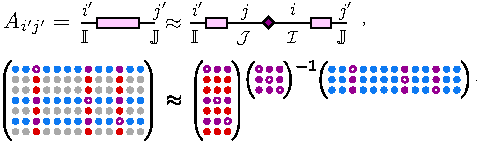
\includegraphics[width=.65\textwidth]{figures/AMCI_IndexSets.pdf}};
		\node[anchor=north east] at (img.north east){\footnotemark};
	\end{tikzpicture}
	\nonumber
\end{gather}

\footnotetext{We introduce here a tensor network diagrammatic representation of the matrix multiplication. The internal connecting solid lines represent summation over the respective matrix indices, according to the \textit{Einstein summation convention}. The external lines represent fixed indices.}

\prettyref{eq:MCI} gives a rank-$\tchi$ approximation of $A$, where $\tchi = \text{dim}\left( \mathcal{I} \right) = \text{dim}\left( \mathcal{J} \right)$. CI is ``only'' a quasioptimal decomposion of $A$ and its accuracy strongly depends on the choice of the pivots; however, contrarily to its optimal counterparts (e.g. SVD), it doesn't require knowing (and saving in memory) the full $M \times N$ matrix to be computed. Let's consider the following example: 
\begin{example}[$5 \times 5$ Correlation matrix]
\label{ex:CIcorrmat}
For classical Harmonic Oscillator 1D chain mode-like vectors: 

\[
\begin{alignedat}{2}      
	\boldsymbol{v} = \frac{\boldsymbol{1}_5}{\sqrt{5}} \qquad \boldsymbol{w} = \frac{(-2,-1,\dots,2)}{2\sqrt{5}}
\end{alignedat}
\]
the corresponding position-position correlation matrix can be ``cross interpolated'' as 

\begin{gather}
	\nonumber \begin{aligned}
		& C  \;=\; \sigma^2 \boldsymbol{v}^T \boldsymbol{v} + \tilde{\sigma}^2 \boldsymbol{w}^T\boldsymbol{w} = \\[.4em]
		& =\frac{1}{115}%
		\begin{tikzpicture}[baseline=-0.5ex,
			every node/.style={inner sep=1pt,font=\small}]
			\matrix (M) [matrix of math nodes,
			nodes={text width=1.8cm, align=center,
			minimum height=1.5em, anchor=center},
			column 1/.style= {nodes={fill=red!30}},
			column 5/.style= {nodes={fill=red!30}},
			row 1/.style= {nodes={fill=yellow!30}},
			row 5/.style= {nodes={fill=yellow!30}},
			row 1 column 1/.style={nodes={fill=orange!30}},
			row 1 column 5/.style={nodes={fill=orange!30}},
			row 5 column 1/.style={nodes={fill=orange!30}},
			row 5 column 5/.style={nodes={fill=orange!30}},
			left delimiter={[},right delimiter={]}, text width=1.8cm,
			ampersand replacement=\&] {
				23\sigma^{2}+72\tilde\sigma^{2} \& 23\sigma^{2}-18\tilde\sigma^{2}
				\& 23\sigma^{2}+12\tilde\sigma^{2}
				\& 23\sigma^{2}-18\tilde\sigma^{2}
				\& 23\sigma^{2}-48\tilde\sigma^{2}\\
				\cdots \& 23\sigma^{2}+{\tfrac92}\tilde\sigma^{2}
				\& 23\sigma^{2}-3\tilde\sigma^{2}
				\& 23\sigma^{2}+{\tfrac92}\tilde\sigma^{2}
				\& 23\sigma^{2}+12\tilde\sigma^{2}\\
				\cdots \& \cdots
				\& 23\sigma^{2}+2\tilde\sigma^{2}
				\& 23\sigma^{2}-3\tilde\sigma^{2}
				\& 23\sigma^{2}-8\tilde\sigma^{2}\\
				\cdots \& \cdots \& \cdots
				\& 23\sigma^{2}+{\tfrac92}\tilde\sigma^{2}
				\& 23\sigma^{2}+12\tilde\sigma^{2}\\
				\cdots \& \cdots \& \cdots \& \cdots
				\& 23\sigma^{2}+32\tilde\sigma^{2}\\
				};
			\draw [decorate, line width=1.5pt,
				decoration = {calligraphic brace,mirror,raise=5pt, amplitude=5pt}] (M.south west) --  (M.south east) node[pos=0.5, below=12pt]{\normalsize $5 \times 5$};
		\end{tikzpicture}
	\end{aligned}
	 \\[1.2em]
	  \approx
	   \underbrace{%
	  C[\mathds{I} , \mathcal{J}]}_{\displaystyle 5 \times 2}
	\,
	\underbrace{%
	  \left[ \begin{array}{>{\columncolor{orange!30}}c>{\columncolor{orange!30}}c}
		\frac{23\sigma^2 + 72\tilde{\sigma}^2}{115} & \frac{23\sigma^2  -48 \tilde{\sigma}^2}{115} \\[0.2em]
		\frac{23\sigma^2 - 48\tilde{\sigma}^2}{115} & \tikzmark{m2}{\frac{23\sigma^2 + 32\tilde{\sigma}^2}{115}}
	  \end{array}\right]^{-1}}_{\displaystyle 2 \times 2}
	  \,
	  \underbrace{%
	  C[\mathcal{I} , \mathds{J}]}_{\displaystyle 5 \times 2}
\end{gather}

with $\sigma$ and $\tilde{\sigma}$ the variances of the two modes and $\mathcal{I} = \{ 1,5\}$ and $\mathcal{J} = \{ 1,5\}$. From the definition of $C$ we can recognize that $\rank{C} = 2$. This property is correctly highlighted by its CI decomposition ($\dim \mathcal{I} = \dim \mathcal{J} = 2$), since, in this particular case, the approximation is exact (cf. \prettyref{prop:CI}-\hyperlink{cond:rankexact}{3.}). The total number of floating point numbers necessary to store the whole matrix in memory is $5 \times 5 = 25$, while for the CI decomposition $5\times 2 \times 2 + 2\times 2 = 24$ are sufficient. It is easy to deduce that the reduction in memory costs becomes less derisory for modes of generic dimension $N$ ($N\times N \gg N \times 2 \times 2 + 2\times 2$ when $N \gg 1$).
\end{example}

From the example above we can evince the computational advantage of CI, however -- in order to make such approximation computationally feasable -- some sort error control is necessary. 
In particular, the error of the CI approximation is related to the \textit{Schur complement} of the matrix to interpolate \cite{Golub96}. 

\begin{definition}[Schur Complement]
	Let us partition a matrix $A\in\mathds{K}^{M\times N}$ ($\mathds{K} = \mathds{R}, \mathds{C}$) in blocks as follows: 

	\begin{equation}
		\begin{bNiceMatrix}[last-row, last-col]
			A_{11} & A_{12} & {\scriptstyle \tchi} \\
			A_{21} & A_{22} & {\scriptstyle M - \tchi} \\
			{\scriptstyle \tchi} & {\scriptstyle N - \tchi}
		\end{bNiceMatrix}.
	\end{equation}
The {\normalfont \textbf{Schur complement}} $[A/A_{11}]$ of $A$ is defined by 
	\begin{equation}
		\label{eq:Schurcomp}
		[A/A_{11}] = A_{22} - A_{21}(A_{11})^{-1}A_{12}.
	\end{equation}
\end{definition}

\begin{proposition}
	\label{prop:CI}
	The following properties hold for a rank-$\tchi$ Cross Interpolation decomposition of a matrix $A$: 

	\begin{enumerate}
		\item the error of CI is given by the Schur complement to the pivot matrix;
		\item the approximation is exact for any $i \in \mathcal{I}$ or $j \in \mathcal{J}$; 
		\item \hypertarget{cond:rankexact} the approximation is exact if $A$ has rank $\tchi$.
	\end{enumerate}
	 
\end{proposition}\vspace{-10pt}
\begin{proof}
	\textit{1.-2.} - The Schur complement is invariant under rows and/or column permutations, therefore let us rearrange $A = A[\mathds{I}, \mathds{J}]$ such that
	\begin{equation*}
		A = \begin{bmatrix}
			A[\mathcal{I}, \mathcal{J}] & A[\mathcal{I}, \mathds{J} / \mathcal{J}] \\
			A[\mathds{I} / \mathcal{I}, \mathcal{J}]  & A[\mathds{I} / \mathcal{I}, \mathds{J} / \mathcal{J}]  
		\end{bmatrix}.
	\end{equation*}
Then, \prettyref{eq:MCI} can be rewritten as 
	\begin{equation*}
		\tilde{A} = \begin{bmatrix}
			A[\mathcal{I}, \mathcal{J}] & A[\mathcal{I}, \mathds{J} / \mathcal{J}] \\
			A[\mathds{I} / \mathcal{I}, \mathcal{J}]  &   A[\mathds{I} / \mathcal{I}, \mathcal{J}] \left(A[\mathcal{I}, \mathcal{J}] \right)^{-1} A[\mathcal{I}, \mathds{J} / \mathcal{J}]
		\end{bmatrix}
	\end{equation*}
	which gives (cf. Ref. \cite{Fernandez2024})
	\begin{equation}
		A - \tilde{A} = \begin{bmatrix}
			0 & 0 \\
			0 & [A/A[\mathcal{I}, \mathcal{J}]]
		\end{bmatrix}
	\end{equation}
\textit{3.} - If $\rank{A} = \tchi$ and $P = A[\mathcal{I},\mathcal{J}]$ is non-singular, then 

\begin{equation}
	\begin{bmatrix}
		A[\mathcal{I}, \mathcal{J}] & A[\mathcal{I},j] \\
		A[i, \mathcal{J}] & A[i,j]
	\end{bmatrix}\qquad \forall\; (i,j) \in \mathds{I} / \mathcal{I} \times \mathds{J} / \mathcal{J}
\end{equation}
is singular, which gives $ A[i,j] = A[i, \mathcal{J}] \left( A[\mathcal{I}, \mathcal{J}] \right)^{-1} A[\mathcal{I},j]$ (cf. App A-B in Ref. \cite{Fernandez2022}). 
\end{proof}

\prettyref{prop:CI} underlines the importance of the choice of the pivots and of the pivot matrix, specifically with the purpose of minimizing the Schur complement $[A/A[\mathcal{I}, \mathcal{J}]]$. Such procedure is equivalent to maximising $\det{A[\mathcal{I}, \mathcal{J}]}$ and is known as the \textit{maximum volume principle} \cite{Goreinov1997}. Moreover, from this analysis, we can also get an intuition about why the CI approximation error is at most $O(\tchi^2)$ times the optimal one (e.g. $\tchi$-truncated SVD error) \cite{Schneider2010}, while requiring only subparts of the original matrix to be known. 

\subsubsection{Partial rank-revealing LU decomposition (prrLU)}
Matrix Cross Interpolation presents itself as a very useful tool when it comes to numerical compression of matrices. Generalization of CI to continuous domains \cite{Schneider2010, Fernandez2022} even allows for reduction of numerical complexity of integration and derivation. Nonetheless, for practical, very complex, calculations, CI starts to fail. Numerical instability issues like rounding errors, ill-conditioning or overflowing \cite{Golub96} easily emerge when CI requires large values of $\tchi$ to be accurate, therefore making the pivot matrix \textit{almost singular}. 

Partial rank-revealing LU (prrLU) \cite{Golub96, Pan2000} matrix decomposition proposes itself as a possible solution for the numerical fragilities of CI. The prrLU provides a more stable, but equivalent approximation of our matrix to decompose. While avoiding any inversion of the pivot matrix $A[\mathcal{I}, \mathcal{J}]$, similarly to CI, prrLU only requires a small subset of matrix's elements to be known. 

We may summarize the main features of prrLU as follows:

\begin{itemize}
	\item prrLU is \textit{rank revealing}, i.e. it allows for the determination of the rank of the decomposed matrix;
	\item prrLU is \textit{partial} (and therefore \textit{controllable}), i.e. the decomposition is stopped after constructing the first $\tchi$ rows of $L$ and columns of $U$, for a fixed $\tchi$;
	\item prrLU is \textit{updatable}, i.e. given pivot lists $\mathcal{I}, \mathcal{J}$ yielding an approximation $\tilde{A}$ of $A$, new rows and columns can easily be added to $\mathcal{I}, \mathcal{J}$ for an improved approximation. 
\end{itemize}

The prrLU implementation relies on the following LU decomposition (easily inferred from \prettyref{eq:Schurcomp}):

\begin{gather}
	\label{eq:SchurLU}
	\begin{bmatrix}
	A_{11} & A_{12} \\
	A_{21} & A_{22}
	\end{bmatrix}
	%\nonumber \\
	=
	\begin{bmatrix}
	L_{11} & 0 \\
	L_{21} & \identity_{22}
	\end{bmatrix}
	\begin{bmatrix}
	A_{11} & 0 \\
	0 & [A / A_{11}]
	\end{bmatrix}
	\begin{bmatrix}
	U_{11} & U_{12} \\
	0 & \identity_{22}
	\end{bmatrix}\\[6pt]
	\nonumber L_{11} = U_{11} = \identity_{11}, \qquad L_{21} = A_{21}A^{-1}_{11}, \qquad U_{12} = A^{-1}_{11}A_{12}
\end{gather} 
From \prettyref{eq:SchurLU} we can already understand where the improved stability of prrLU comes from: no matrix inversion is computed directly! The general prrLU routine proceeds as outlined below:  

\begin{algorithm}[H]
	\caption{Partial rank revealing LU}
	\label{alg:prrLU}
    \SetKwFunction{findBestPivot}{findBestPivot}
	\SetKwFunction{LowerTriangular}{LowerTriangular}
	\SetKwFunction{strictlyUpperTriangular}{strictlyUpperTriangular}
    \SetKwInOut{KwIn}{Input}
    \SetKwInOut{KwOut}{Output}

    \KwIn{$A\in\mathds{K}^{M\times N}$ matrix, max rank $\tchi$ and tolerance $\varepsilon$. }
    \KwOut{Rows permutation $\Pi_r$, columns permutation $\Pi_c$, $L$, $U$, $N_{pivots}$}

    $\Pi_r\leftarrow(1,\dots,M)$,\quad $\Pi_c\leftarrow(1,\dots,N)$,\quad 
	$n\leftarrow0$,\quad $\varepsilon_{LU} \leftarrow \varepsilon$\;

	\While{$n<\min(\tchi,\,M,\,N)$}{
		$n\leftarrow n+1$\;
		$(r^\star,c^\star)\leftarrow 
		\findBestPivot\!\bigl(A[n\!:\!N, n\!:\!M]\bigr)$\tcp*[f]{current positions}\;
		swap rows $n\leftrightarrow r^\star$ in $A$ and $\Pi_r$\;
		swap cols $n\leftrightarrow c^\star$ in $A$ and $\Pi_c$\;
		$\varepsilon_{LU} \leftarrow |A_{n,n}|$\;
		\If(\tcp*[f]{error test}){$n>0$ \KwSty{and} $\varepsilon_{LU} <\varepsilon$}{
			\textbf{break}\;
		}	
	}
	
	$L\leftarrow\LowerTriangular\bigl(A[:,\,1\!:\!n]\bigr)$\;
	$U\leftarrow\strictlyUpperTriangular\bigl(A[1\!:\!n,\,:]\bigr)$\;
	\Return{$(\Pi_r,\,\Pi_c,\,L,\,U,\,n)$}\;
\end{algorithm}

By iteratively applying \prettyref{eq:SchurLU} on the lower-right block of the internal matrix, while limiting $A_{11}$ to a $1\times 1$ submatrix, \prettyref{alg:prrLU} allows us to obtain an approximation of the form 

\begin{equation}
	\label{eq:prrLUCI}
	A = LDU + \begin{bmatrix}
		0 & 0\\
		0 & [A/A[\mathcal{I}, \mathcal{J}]]
	\end{bmatrix} = \tilde{A} + \textrm{err.},
\end{equation}

perfectly equivalent to \prettyref{eq:MCI} (cf. Ref. \cite{Fernandez2024}), where $D$ is a diagonal matrix containing -- after iterative permutations -- the first $\tchi$ optimal pivots of $A$.
Some remarks about \prettyref{alg:prrLU} are in order: 
\begin{itemize}
	\item the implementation of prrLU is based upon the search of a good \textit{pivot} (\texttt{findBestPivot}). Through the \textit{maxvol principle}, a good pivot is defined as one that maximises the volume of the submatrix $A[\mathcal{I}, \mathcal{J}]$ ($\equiv A_{11}$ after permutation). The iterative application of \prettyref{eq:SchurLU} reduces the optimization pivot to the largest element of the submatrix $A[n\!:\!N,n\!:\!M]$ at iteration $n$;
	\item different strategies can be implemented for pivot searching; a naive approach consists in a \textit{full search} scheme scanning the entire submatrix. $\order(MN)$ poor scaling of the naive implementation renders prrLU computationally inefficient. \textit{Rook search} \cite{Poole2000} and \textit{block rook search} \cite{Fernandez2024} are cleverer and cheaper approaches, with comparable robutstness and convergence, but reduced computational cost $\order(\max\left(M,N\right))$;  
	\item the matrix elements explored during \textit{rook search} are sufficient to perform prrLU of $A$. Therefore, prrLU yields compressibility features similar to those of CI (see Example \ref{ex:CIcorrmat}). For this reason, prrLU can also be applied to 2-dimensional continuous functions discretized on a grid, whose full structure is uknown a priori; 	
	\item the absolute error of the prrLU approximation is reduced to the modulus of the last inserted pivot, as one can understand from \prettyref{alg:prrLU}. The reason behind this is that we intend to minimize $\parallel\! A - \tilde{A}\!\parallel_{\infty} = \parallel\![A/A[\mathcal{I}, \mathcal{J}]] \!\parallel_{\infty}$ which is bounded by $\parallel\! A[n_{\textrm{end}}\!:\!N, n_{\textrm{end}}\!:\!M]\!\parallel_{\infty}$ of the last iteration.  
\end{itemize}


\subsection{Tensor Cross Interpolation}

Tensor Cross Interpolation is a generalization of matrix Cross Interpolation -- and therefore prrLU (see \prettyref{eq:prrLUCI}) -- to $\mathcal{L}$-dimensional tensors $\mathcal{T}$. Similarly to prrLU, TCI progressively uncovers the \textit{low rank} structure of a given tensor, rendering a very functional approximation of the input. The main struggle of TCI routines revolves around bookkeeping of tensor indices -- the \textit{pivots} -- necessary for a correct approximation. 
Let us then introduce some useful notation: 
\begin{itemize}
	\item $\mathcal{T}_{\boldsymbol{\sigma}} \in \mathds{K}^{I_1\times I_2\times \dots \times I_\mathcal{L}}$ is the TCI input tensor, with indices $\boldsymbol{\sigma} \in I_1\times I_2\times \dots \times I_\mathcal{L}$ ($\dim I_i = d_i \footnotemark $); $\mathcal{\widetilde{T}}_{\boldsymbol{\sigma}} \in \mathds{K}^{I_1\times I_2\times \dots \times I_\mathcal{L}}$ is the resulting interpolated tensor:
	\begin{align}
		\label{eq:globTTensor}   
	 \mathcal{T}_{\boldsymbol{\sigma}} 
	 = \raisebox{-5mm}{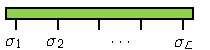
\includegraphics{figures/fnatural_short.pdf}} \approx  \mathcal{\widetilde{T}}_{\boldsymbol{\sigma}} \, ; 
	 \end{align}
	\footnotetext{For most application $d_i=d\; \forall i$, with fixed $d$. }
	\item $\mathds{I}_\ell = I_1\times I_2\times \dots \times I_\ell$ and $\mathds{J}_\ell = I_\ell\times I_2\times \dots \times I_\mathcal{L}$\footnotemark denotes, respectively, the set of all \textit{row multi-indices} and \textit{column multi-indices} up to and from site $\ell$ (e.g. $i \in \mathds{I}_\ell$, $j \in \mathds{J}_\ell$ implies $i = (\sigma_1, \dots, \sigma_\ell)$, $j = (\sigma_\ell, \dots, \sigma_\mathcal{L})$);
	\item $\mathcal{I}_\ell \subseteq \mathds{I}_\ell$ and $\mathcal{J}_\ell \subseteq \mathds{J}_\ell$ are, respectively, lists of \textit{pivot rows} and \textit{pivot columns} and contain only a subset of the total multi-indices, the \textit{pivots};
	\item the following objects represent \textit{slices} of the original tensor:
	\begin{gather}
		\nonumber [P_\ell]_{ij} = \mathcal{T}_{i\oplus j} 
		= \raisebox{-5mm}{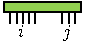
\includegraphics{figures/PtensorWithLegsNoell.pdf}} \, , \quad [T_\ell]_{i\sigma j} \equiv \mathcal{T}_{i\oplus (\sigma) \oplus j} 
		= \raisebox{-5mm}{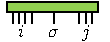
\includegraphics{figures/TtensorWithLegsNoell.pdf}} \, ,\\[6pt] 
		[\Pi_\ell]_{i\sigma \sigma'j} \equiv  \mathcal{T}_{i\oplus (\sigma,\sigma') \oplus j}
	= \raisebox{-5mm}{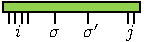
\includegraphics{figures/PiTensorWithLegsNoell.pdf}} \, ,
	\label{eq:Tslices} 
	\end{gather}
	where $\oplus$ is the index \textit{concatenation operation}, i.e. $i\oplus j \equiv (\sigma_1, \dots, \sigma_\mathcal{L})$, for $i\in \mathds{I}_\ell$ and $j \in \mathds{J}_{\ell+1}$. 

\end{itemize}

\footnotetext{$\mathds{I}_\mathcal{L} = \mathds{J}_1$ corresponds to the full set of tensor indices, i.e. $\boldsymbol{\sigma} \in  \mathds{I}_\mathcal{L} = \mathds{J}_1\; \forall \boldsymbol{\sigma}$}

The main purpose of TCI is perform the decomposition of a given tensor using only few elements of (few calls to) the tensor $\mathcal{T}_{\boldsymbol{\sigma}}$. \prettyref{fig:TCIalg} below summarizes the main steps 
of the TCI routine. 

\begin{figure}[ht!]
	\centering
	\includegraphics[width=\textwidth]{figures/TCI.pdf}
	\caption{Main steps of the TCI algorithm. $a)$ A set of indices such that $\mathcal{T}_{\hat \sigma} \neq 0$ is chosen randomly from the configuration space. Pivot lists are constructed from the initial multi-indices set. $b)$ A first sweep is performed for an initial Matrix Product State representation of our tensor $\mathcal{T}$. $\Pi_\ell$ tensor slices of the form in \prettyref{eq:Tslices} are constructed from the initial pivot lists $\mathcal{I}_\ell$ and $\mathcal{J}_\ell$. prrLU is then perfomed on the ``matricized'' version of $\Pi_\ell$ -- $\bigl[\Pi_\ell\bigr]_{(i_{\ell -1}, \sigma_\ell) (\sigma_{\ell+1}, j_{\ell +2})}$ -- and new pivots $\mathcal{I}'_\ell$ and $\mathcal{J}'_\ell$ are added to the initial lists. This second step resembles the naive approach introduced in Ref. \cite{Fernandez2022} for pedagogical purposes, as well as the well-established SVD-based MPS tensor decomposition (cf. Ref. \cite{vonDelftTNNotes}). $c)$ Sweeping back and forth through index pairs -- $\sigma_\ell, \sigma_{\ell +1}$ -- the 2-dimensional slices $\Pi_\ell$ are reconstructed from the current local pivot lists and prrLU-compressed again, in order to improve the choice of the initial \textit{pivots} and the approximation $\widetilde{\mathcal{T}}$. This last step is performed until convergence.}
	\label{fig:TCIalg}
\end{figure}

The algorithm depicted in \prettyref{fig:TCIalg} represents what is usually referred to as the \textit{2-site TCI algorithm} \cite{Fernandez2024}. The \textit{2-site} annotation underlies the fact that the approximation $\widetilde{\mT}$ is only built through two-dimensional slices of $\mT$. This version of the implementation relies on two main ingredients: the partial rank-revealing LU and the \textit{interpolation} properties of TCI. Whilst we extensively introduced the former in the previous section, a few comments are necessary about the latter. Let us first take a step back and briefly introduce the concept of \textit{nesting conditions}. The list of pivot rows (columns) is said be \textit{left- (right-) nested} if the following condition holds \cite{Oseledets2011, Dolgov2020}:

\begin{equation}
	\label{eq:Nesting}
	\mI_0 <  \mI_1  < \ldots < \mI_{\ell} ,\quad (\mJ_{\ell} > \mJ_{\ell+1} > \ldots > \mJ_{\mL+1} ,)
\end{equation}

where $\mI_{\ell -1 } <\mI_\ell$,  if
$\mI_\ell \subseteq \mI_{\ell -1 } \times 
I_\ell $ ($\mJ_{\ell} > \mJ_{\ell +1}$,  if
$\mJ_\ell \subseteq J_\ell \times \mJ_{\ell + 1 }$). The pivot lists are \textit{fully left- (right-) nested} if $\ell = \mL - 1 (=2)$. \textit{Full nesting} is achieved when both full right- and left-nesting is respected.

The benefit of nesting condition is the already mentioned interpolation characteristics of TCI (we refer the reader to Ref. \cite{Fernandez2022, Fernandez2024} for proofs and a more detailed explanation). In fact, when pivots are right-nested up to $\ell -1$ and left-nested from $\ell +2$ on, then
\begin{equation}
	\label{eq:ErrorPiIsErrorT}
	\bigl[\varepsilon_\Pi\bigr]_{i_{\ell-1}\sigma_\ell \sigma_{\ell +1} j_{\ell +2 }} \equiv \bigl[ \Pi_\ell - \widetilde{\Pi}_\ell\bigr]_{i_{\ell-1}\sigma_\ell \sigma_{\ell +1} j_{\ell +2 }} 
	= 
   \bigl[ \mT-\widetilde{\mT}\bigr]_{i_{\ell-1}\sigma_\ell \sigma_{\ell +1} j_{\ell+2}},
 \end{equation}
where 

\begin{equation}
	\raisebox{-5mm}{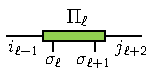
\includegraphics{figures/Pi_FactorizationLeft.pdf}} 
	\mathrel{\stackrel{\makebox[0pt]{\mbox{\normalfont\tiny prrLU}}}{\approx}}
		 \raisebox{-5mm}{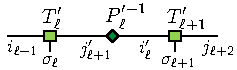
\includegraphics{figures/Pi_FactorizationRightPrime.pdf}} = \widetilde{\Pi}_\ell.
	\label{eq:Piapprox}
\end{equation}
In \prettyref{eq:ErrorPiIsErrorT} and \prettyref{eq:Piapprox} (and also \prettyref{fig:TCIalg}), $\Pi_\ell$ is the exact slicing of $\mT$, reconstructed from the current set of local pivots $\mI_{\ell -1}$ and $\mJ_{\ell +2}$; $\widetilde{\Pi}_\ell$ is its approximation through prrLU. \prettyref{eq:ErrorPiIsErrorT} allows us to define a consitent local error concept, granting the TCI algorithm of a form error control. In fact, step $c)$ in \prettyref{fig:TCIalg} is performed until the \textit{bare error} $\bigl| \Pi_\ell - \widetilde{\Pi}_\ell\bigr|_{i_{\ell-1}\sigma_\ell \sigma_{\ell +1} j_{\ell +2 }}$ is below a fixed tolerance $\varepsilon$. Minimizing the local error means, according to \prettyref{alg:prrLU} and the \textit{maxvol principle} \cite{Dolgov2020}, searching for the largest elements of the tensor $\bigl| \Pi_\ell - \widetilde{\Pi}_\ell\bigr|$, in order add new pivots that yields the largest improvement to the local accuracy according to the $\|\cdot \|_{\infty}$ norm. The TCI routine is stopped when the condition $\|\mT - \widetilde{\mT}\|_{\infty} < \varepsilon$ is met in each local slice, for the minimal set of pivots possible. 

TCI representation is defined by the selected lists $\mI_\ell$ and $\mJ_\ell$ $\forall \ell$, so an accurate interpolation amounts to optimizing this selection. The TCI routine, as mentioned at the beginning of this work, belongs to the class of ``active machine learning'' algorithms \cite{Settles2012}, as it tries to uncover the low-rank structure of a given tensor $\mT$ by actively requesting configurations that will better improve its MPS unfolding. Similar to machine learning (ML), different techniques exist to improve the modelling of our data set (e.g. for ML: data augmentation, weighting, prompt engineering etc.).
In our case, alongside the local pivot searching strategies -- \textit{rook search}, \textit{block rook search} and \textit{full search} -- higher level techniques exist to improve the global approximation of our tensor. The 2-site TCI can be run in \textit{reset mode} that, in contrast to the \textit{accumulative mode}, only adding new pivots to the local lists, recomputes the full lists $\mI_\ell$ and $\mJ_{\ell+1}$ at each prrLU step. This allows us to discard sub-optimal pivots that were inserted in the pivots lists during the initial exploration of the configuration space. \textit{Global pivot proposals}, similar to multi-start approaches in ML \cite{Loshchilov2017}, allow to incorporate prior information about the tensor $\mT$ through a clever choice of the initial configurations $\boldsymbol{\hat  \sigma}$ (see \prettyref{fig:TCIalg}$.a$), such that the whole configuration space is uniformly explored. \textit{0-site} and \textit{1-site TCI} focused on prrLU optimization of the $T$ and $P$ slices (\prettyref{eq:Tslices}) help restoring full nesting and removing ill-conditioned pivots, respectively.

The above procedures all try to target TCI \textit{ergodicity} issues that arise in different implementations. In particular, \textit{sparse or symmetric tensors} and \textit{narrow peaked multivariate} functions are the main weaknesses for TCI employment. Most common TCI applications don't require any further resolution method, however, as we will understand in the rest of this work, there exist many other, especially if modelling very extreme-conditioned physical systems, that call for additional improvements.

\begin{table}[ht!]
	\centering
	\small                       % shrink the font a bit (optional)
	\setlength{\tabcolsep}{4pt}  % tighter column separation (optional)
  
\begin{adjustbox}{max width=\textwidth} 
	\begin{tabular}{|c|c|c|c|c|}
	\hline 
	action & \multicolumn{2}{c|}{variant} & calls to $\mT_{\boldsymbol{\sigma}}$ & algebra cost\tabularnewline
	\hline 
	\hline 
	\multirow{4}{*}{iterate} & rook piv. & 2-site & $\order(\chi^{2}dn_{\text{rook}}\mL)$ & $\order(\chi^{3}dn_{\text{rook}}\mL)$\tabularnewline
	\cline{2-5} \cline{3-5} \cline{4-5} \cline{5-5} 
	 & full piv. & 2-site & $\order(\chi^{2}d^{2}\mL)$ & $\order(\chi^{3}d^{2}\mL)$\tabularnewline
	\cline{2-5} \cline{3-5} \cline{4-5} \cline{5-5} 
	 & full piv. & 1-site & $\order(\chi^{2}d\mL)$ & $\order(\chi^{3}d\mL)$\tabularnewline
	\cline{2-5} \cline{3-5} \cline{4-5} \cline{5-5} 
	 & full piv. & 0-site & 0 & $\order(\chi^{3}\mL)$\tabularnewline
	\hline 
	achieve full nesting & \multicolumn{2}{c|}{} & $\order(\chi^{2}d\mL)$ & $\order(\chi^{3}d\mL)$ \tabularnewline
	\hline 
	add $n_{p}$ global pivots & \multicolumn{2}{c|}{} & $\order\bigl((2\chi+n_{p})n_{p}\mL\bigr)$ & $\order\bigl((\chi+n_{p})^{3}\mL\bigr)$\tabularnewline
	\hline 
	\multirow{3}{*}{compress tensor train} & \multicolumn{2}{c|}{SVD} & \multirow{3}{*}{0} & \multirow{3}{*}{$\order(\chi^{3}d\mL)$}\tabularnewline
	\cline{2-3} \cline{3-3} 
	 & \multicolumn{2}{c|}{prrLU} &  & \tabularnewline
	\cline{2-3} \cline{3-3} 
	 & \multicolumn{2}{c|}{CI} &  & \tabularnewline
	\hline 
	\end{tabular}
\end{adjustbox}

\caption{Computational cost of the main TCI routines. Full nesting routines are fundamental to restore nesting and, with it, interpolation properties for our Tensor Train approximation. Rook pivoting and full pivoting are different possible choices for the pivot search in prrLU/CI subroutines. $n_{rook}$ corresponds to the average number of rook search moves necessary to find an optimal local pivot ($n_{rook} < 5$ for most applications). The table is taken directly from Ref. \cite{Fernandez2024}.}
\label{tab:cost}
\end{table}	

Tensor Cross Interpolation, as the $\mL$-dimensional extension of CI, conserves its compression properties. The approximation is systematically controlled by $\chi$, where $\chi = \max_{\ell} \chi_\ell$ is the \textit{rank} of the tensor $\mT$ with $\chi_\ell = \dim \mI_\ell = \dim \mJ_{\ell +1}$, and so TCI computational resources' scaling strongly depends on $\chi$.
The number of function calls necessary for the MPS unfolding $\widetilde{\mathcal{T}}$ of $\mathcal{T}$ is $\order (\chi^2d\mathcal{L})$ compared to the $d^\mathcal{L}$ ($= |\mathds{I}_\mL| = |\mathds{J}_1|$) of its SVD counterpart, where $d$ is the local configuration space dimensionality. Such an exponential advantage is obtained by fully specifying only $\order (\chi^2\mathcal{L})$ number of \textit{pivots} from the original tensor. The algebra cost ($\sim$ computational time) of the algorithm scales then as $\order (\chi^3d\mathcal{L})$. Scaling of the main TCI routines provided by the \texttt{TensorCrossInterpolation.jl} $\julia$ library \cite{TensorCrossInterpolation.jl} is detailed in \prettyref{tab:cost}. From this analysis, as well as from Example \ref{ex:Ldimfunc}, we can understand that TCI possess incredible memory saving power compared to other MPS unfolding routines.
\begin{example}[$\mL$-dimensional function]
Inspiring ourselves from \cite{Fernandez2024}, we construct an example to exhibit TCI compression capabilities. Let us consider the following $\mL$-dimensional function: 

\begin{equation}
	f(\boldsymbol{x}) = 
   \frac{2^\mL}{1 + 2 \sum^\mL_{\ell=1} x_\ell} .
   \label{eq:Ldimfunc}
\end{equation}

As one can easily understand, such a continuous function can be numerically represented by a tensor $\mathcal{F}_{\bsigma}$ through grid discretization over a preferred domain. In our case, we take a 61 point Gauss-Kronod type of grid, over the $[0,1]^\mL$ hypercube for this exercise. What this means in practice is that $\mathcal{F}_{\bsigma} \in \mathds{R}^{I_1\times\dots\times I_\mL}$ and $\dim I_i = d = 61$. TCI approximation of $\mathcal{F}_{\bsigma}$ renders a tensor $\widetilde{\mathcal{F}}_{\bsigma}$ with only a limited number of calls to the original function $f(\boldsymbol{x})$, as depicted in \prettyref{fig:TCIscaling} below. 

\prettyref{fig:TCIscaling} perfectly documents the reduced memory footprint required from the TCI representation of functions up to 20 dimensions. Exponential scaling of memory requirements, necessary to store the total $61^\mL$ number of tensor elements of $\mathcal{F}_{\bsigma}$, is replaced by an $\chi$ dependent polynomial scaling. Moreover, as one can understand from the bottom right plot in \prettyref{fig:TCIscaling}, out of the total $61^2$ ($\mL=2$) Gauss-Kronod grid points, only $49$ are actually required for a nearly optimal approximation of $f$, therefore limiting the bond dimension $\chi$ of our tensor train to $\chi = 7$ and with that the number of total parameters. 
\begin{figure}[ht!]
		\centering
		\includegraphics[width=0.9\textwidth]{figures/TCI_memory_scaling+heatmap.pdf}
		\caption{TCI approximation of $f(\boldsymbol{x})$ in \prettyref{eq:Ldimfunc} after discretization on a $\mL$-dimensional 61 point Gauss-Kronod grid. \textit{On the left}: number of total floating point elements stored in the compressed tensor $\widetilde{\mathcal{F}}_{\bsigma}$ as a function of $\mL$ (blue line). The ``worst-case-scenario'' scaling $d^\mL$ and the theoretical scaling $\order (\chi^2d\mathcal{L})$ are also represented (green and red dashed line, respectively). \textit{Top right:} heatmap of the $\mL = 2$ approximation $\widetilde{\mathcal{F}}_{\bsigma}$ over the $61\times61$ Gauss-Kronod grid subset of $[0,1]\times[0,1]$. \textit{Bottom right:} heatmap of the $\mL = 2$ original function  $f(\boldsymbol{x})$ over the domain $[0,1]\times[0,1]$. The red dots represent the location of the \textit{pivot} values exploited for the TCI approximation.
		}
		\label{fig:TCIscaling}
	\end{figure}
\label{ex:Ldimfunc}
\end{example}

The advantages of the TCI algorithm are not purely limited to function approximation. A very obvious application of TCI reduces to the computation of very large and complex integrals. Detailed examples of this particular employment of TCI are provided in Ref. \cite{Fernandez2022, Fernandez2024, Dolgov2020}. TCI-based integration significantly outperform Monte-Carlo and quasi-Monte-Carlo methods in many occasions and the reasons behind it are diverse. 

Condider the following integral:
\begin{equation}
	I \equiv \int d\boldsymbol{x} \ f(x_1,\dots,x_\mL),
	\label{eq:LdimIntegral}
\end{equation}
through numerical discretization it can be reduced to 
\begin{equation}
	I \approx \sum_{\bsigma} \mathcal{F}_{\bsigma} ,\quad \; \mathcal{F}_{\bsigma} = f(\boldsymbol{x}(\bsigma))
	\label{eq:LdimapproxIntegral}
\end{equation}
where $\boldsymbol{x}(\bsigma)$ is our discretization grid. If we decide to perform TCI unfolding of our numerical tensor $\mathcal{F}_{\bsigma}$ before the integration, \prettyref{eq:LdimapproxIntegral} then reads
\begin{equation}
	\sum_{\bsigma} \mathcal{F}_{\bsigma} \approx \prod_{\ell=1}^\mL \sum^{d_\ell}_{\sigma_\ell = 1} T^{\sigma_\ell}_\ell P^{-1}_\ell \; \;\footnotemark
	\label{eq:LdimTCIIntegral}
\end{equation}
replacing one $\mL$-dimensional integral by $\chi^2\mL$ exponentially easier problems. Moreover, if the rank of the MPS unfolding of the integrand remains roughly constant as the number of dimensions increases, then the gain in favor of TCI increases exponentially. Given the numerical simplicity of the algebra operations in \prettyref{eq:LdimTCIIntegral}, the bottleneck of integration operations is limited to finding the right TCI approximation of the integrand, bounding the scaling to a \textit{polynomial} cost of $\order (\chi^2d\mathcal{L})$. 

\footnotetext{$P$ and $T$ slices are here considered as ($\sigma_\ell$-dependent) matrices. Summation over common indices is implied. $P_{\mL} = [1]$.}

The above achievement of TCI relies on the following property of continuous functions:
\begin{definition}
	A function $f$ is {\normalfont \textbf{almost separable}} \cite{Fernandez2024} or {\normalfont \textbf{$\boldsymbol{\varepsilon}$-factorizable}} \cite{Fernandez2022} if its tensor approximation $\mathcal{F}$ is low-rank.
	\label{def:separfunc}
\end{definition}

For this class of functions the advantage of TCI integration over more standard approaches -- like Monte Carlo sampling -- is incomparable (cf. $1/N_{\text{eval}}^4$ vs. $1/\sqrt{N_{\text{eval}}}$ convergence for $N_{\text{eval}}$ function evaluations in Fig. 2 Ref. \cite{Fernandez2024}). Moreover, for computations revolving around quantum mechanical systems, TCI does not suffer from the \textit{``sign problem''} that always goes along with sampling methods such as Quantum Monte Carlo, especially when they try to deal with integration of highly-oscillating functions. TCI performs exteremely well even when dealing with functions oscillating simultaneously on very different scales. Consequently, we can understand that the limiting factor of TCI (rank of the $\varepsilon$-factorization) is entirely orthogonal
to that of sampling methods.

If the user intends to employ TCI purely to perform complex integrations, the definition of an \textit{environment-aware error} (from \prettyref{eq:ErrorPiIsErrorT} and \prettyref{eq:LdimTCIIntegral}) might turn out to be very useful

\begin{gather}
	\nonumber\bigl[\varepsilon^{\text{env}}_\Pi\bigr]_{i_{\ell-1}\sigma_\ell \sigma_{\ell +1} j_{\ell +2 }}\equiv |L_\ell R_\ell| \bigl[\varepsilon_\Pi\bigr]_{i_{\ell-1}\sigma_\ell \sigma_{\ell +1} j_{\ell +2 }} \\
	L_\ell = \prod_{\bar{\ell}=1}^{\ell -1} \sum^{d_{\bar{\ell}}}_{\sigma_{\bar{\ell}} = 1} T^{\sigma_{\bar{\ell}}}_{\bar{\ell}} P^{-1}_{\bar{\ell}} \quad R_\ell = \prod_{\bar{\ell}=\ell +2}^{\mL} \sum^{d_{\bar{\ell}}}_{\sigma_{\bar{\ell}} = 1}  P^{-1}_{\bar{\ell}-1}T^{\sigma_{\bar{\ell}}}_{\bar{\ell}}.
	\label{eq:envError}
\end{gather}
Substituting the usual definition of local  error $\varepsilon_\Pi$ with the environment error function $\varepsilon^{\text{env}}_\Pi$ allows the TCI routing to be more integral-focused, outperforming the standard implementation when it comes to integral error convergence. By selecting pivots not only based on the absolute value of the integrand but also taking into account a specific point's volume contribution to the integral,  $\varepsilon^{\text{env}}_\Pi$ allows for more precise computations of complex integrals particularly for multi-scaled functions \cite{Fernandez2022}.   


\note{Tensor Cross Interpolation}{Main paper: \cite{Fernandez2024}, Main TCI ref: \cite{Oseledets2010}, function learning, \textit{maxvol} principle \cite{Dolgov2020}, exact if $\rank{TT} = \chi$ like MCI (see Naive Approach \cite{Fernandez2022}), \textit{rank-revealing} (only slow convergence for high rank); separation of pivot exploration and tensor update could be beneficial (see Monte Carlo \textit{space configuration enlargment}); SVD stability issues compared to prrLU}\\

\noindent\note{Nice sentences}{ Tensor network methods offer a new appraoch to high-dimensional integration.TCI has a very peculiar position among other tensor network algorithms: it provides
an automatic way to map a very large variety of physics and applied mathematics problems onto the MPS toolbox. }\\

\noindent\note{General references}{\cite{Oseledets2010, Oseledets2011, Savostyanov2014, Savostyanov2011, Dolgov2020}}\\
\note{Open questions}{Generality of $\epsilon$-factorizability property}

\subsection{The Quantics Representation: QTCI}



\note{QTCI}{Discards weak entanglement between different scales; works well for scale-separated, non-irregular functions; $O(\mathcal{L} \log N )$ ($N \stackrel{?}{=} 2^R $) quantics approximation scaling 4 $\to$ logarithmic scaling in the number of grid points \cite{Khoromskij2011}; exponentially high resolution; low-rank scale separated structure revealed through TCI + quantics }\\

\noindent \note{Nice Sentences}{Numerical computations with multivariate functions typically involve a compromise between two contrary desiderata: accurate resolution of the functional dependence, versus parsimonious memory usage. If the function variables are strongly entangled then using the interleaved quantics representation can lead to a more compressible tensor.}\\

\noindent \note{General references}{\cite{Oseledets2009} (quantics and interleaved representation) }\\

\noindent \note{Applications}{Approximation and manipulation of correlation functions for quantum many body systems \cite{Hiroshi2023}; compression of imaginary-time propagators in the Frobenious norm \cite{Takahashi2025}; diagrammatic non-equilibrium many-body Green’s function-based calculations \cite{Murray2024} $\to$ better scaling of resourses for higher precisions $R$ or longer times }\\

\noindent \note{Open questions 
}{When does a multivariate function admit low-rank representation? }





\section{Computational Fallbacks: Localised Functions}

\begin{figure}[ht!]
	\caption{2D: Heatmap + error Heatmap of TCI approximation of a very localised function with different zoomings  }
\end{figure}

\subsection{Localised Function and Memory Consumption}

\begin{figure}[ht!]
	\caption{1D: plot of different patch subdivision and relative bond dimension per patch for each division (like patching paper)  }
\end{figure}

\begin{figure}[ht!]
	\caption{2D: Bond dimension vs bond for each of the zoomings and for one of the more trivial parts of the function. }
\end{figure}

